\section{Arquitetura Computacional}
\label{sec:arquitetura}

A arquitetura computacional do VIDA foi desenvolvida de forma distribuída e modular, sendo composta por três níveis de processamento: um microcontrolador ESP32, um computador embarcado Odroid e um notebook. Essa organização distribui as funções de aquisição, controle, localização e navegação entre dispositivos com capacidades computacionais distintas e estabelece uma infraestrutura escalável e capaz de receber novos subsistemas. Embora os algoritmos atualmente implementados sejam computacionalmente leves, a manutenção de um nível adicional de processamento permite validar a comunicação entre dispositivos e prepara a plataforma para aplicações futuras mais exigentes, como percepção visual, planejamento de movimento e inteligência artificial.

\subsection{Comunicação e Integração dos Subsistemas}

A integração dos três níveis de processamento é realizada por meio do ROS~2 Humble, cuja arquitetura se basea em nós, tópicos e serviços e permite a comunicação entre componentes distribuídos \citep{Macenski2022}. A Figura~\ref{fig:arquitetura_computacional} apresenta a organização geral da arquitetura e as principais interfaces de comunicação entre os dispositivos.

\begin{figure}[htb]
    \centering
    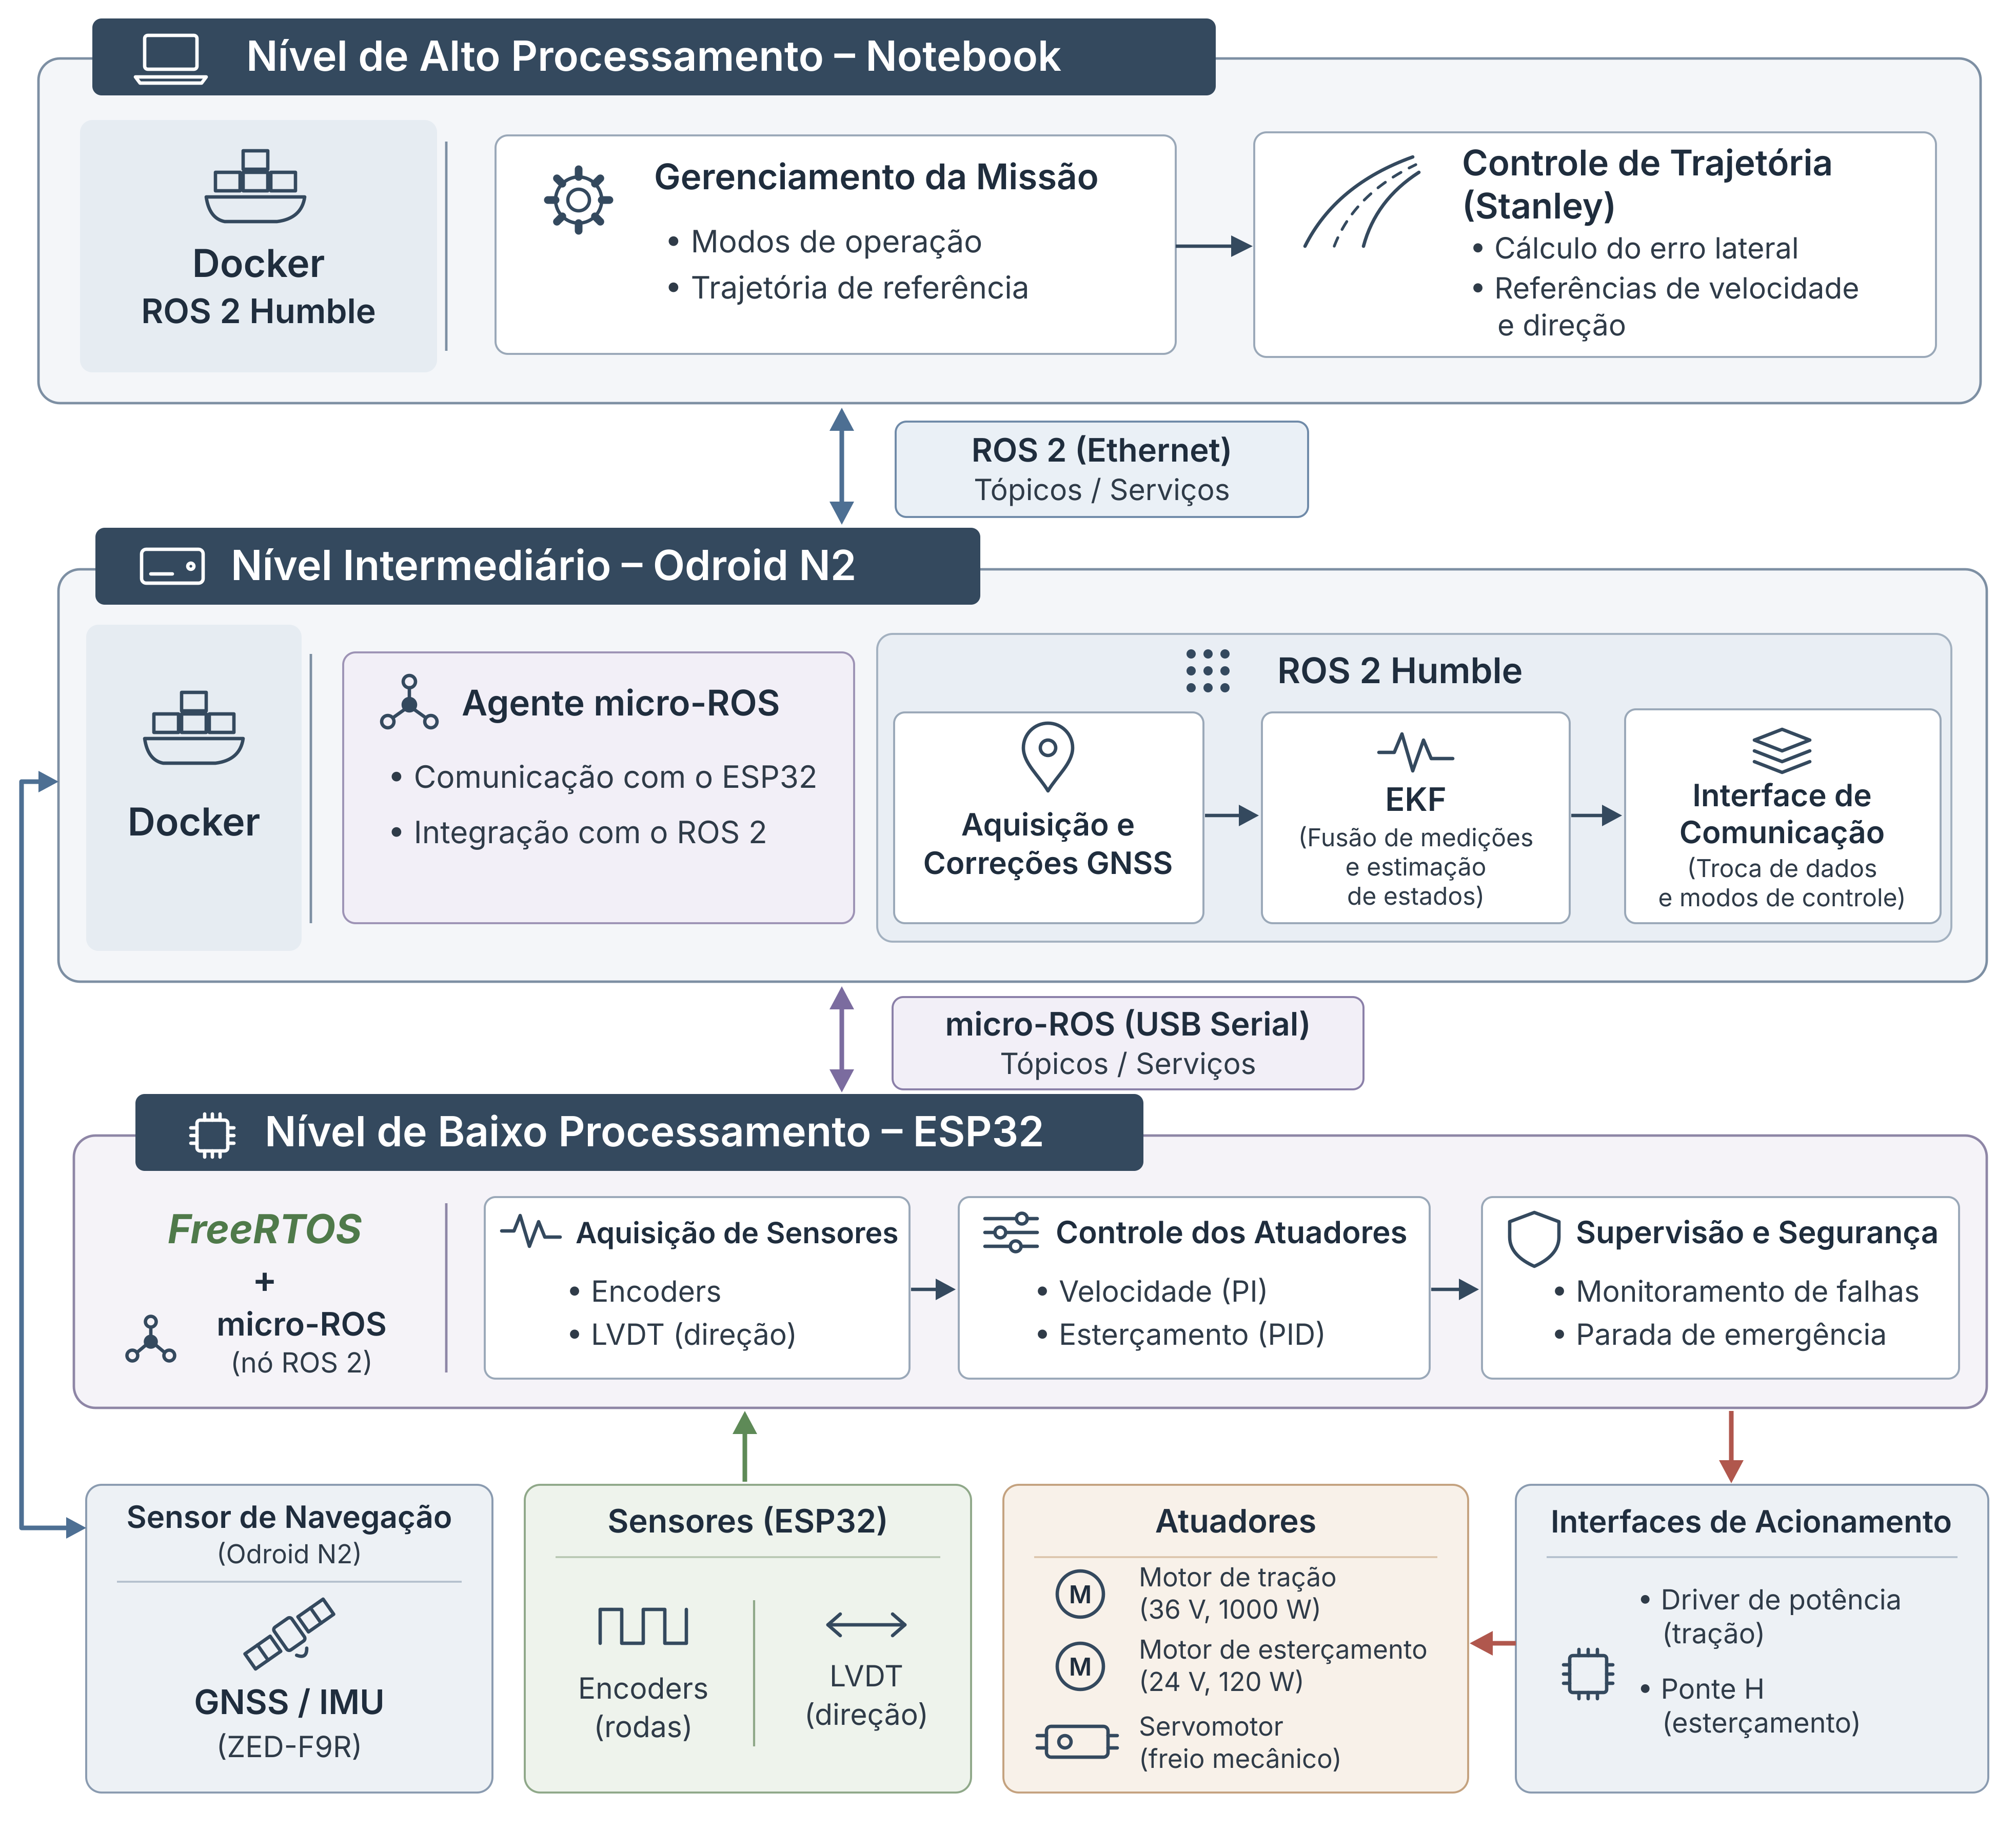
\includegraphics[width=\columnwidth]{Imagens/Arquitetura computacional.png}
    \caption{Arquitetura computacional plataforma VIDA. Fonte: Elaborado pelo autor.}
    \label{fig:arquitetura_computacional}
\end{figure}

A comunicação entre o ESP32 e a Odroid é realizada por uma conexão serial USB a 921\,600~bit/s, utilizando o micro-ROS e o protocolo XRCE-DDS. O agente micro-ROS executado na Odroid estabelece a ponte entre o microcontrolador e a rede DDS do ROS~2.

A Odroid e o notebook são conectados por um cabo Ethernet ponto a ponto, com endereçamento IP fixo. Por essa conexão trafegam as mensagens DDS entre os nós ROS~2 dos dois dispositivos, incluindo os estados estimados, as informações de navegação e as referências de controle. Ambos utilizam a implementação Fast DDS, configurada para transporte exclusivamente por UDP, no mesmo domínio ROS~2.

Adicionalmente, o notebook compartilha com a Odroid, por tradução de endereços de rede (NAT), a conexão com a Internet obtida por rede sem fio. Esse compartilhamento fornece o acesso necessário para que o cliente NTRIP receba as correções RTK.

A utilização de containers Docker na Odroid e no notebook padroniza os ambientes de execução, encapsulando as dependências dos componentes ROS~2 e reduzindo problemas de compatibilidade com os sistemas hospedeiros.

Dessa forma, a arquitetura implementada estabelece uma infraestrutura modular para aquisição, controle, localização e navegação, permitindo a comunicação entre componentes executados em diferentes unidades de processamento e preservando a possibilidade de redistribuição e expansão das funções computacionais da plataforma.

\subsection{Nível de Baixo Processamento -- ESP32}

O nível de baixo processamento é constituído por um microcontrolador ESP32, responsável pela aquisição dos sensores de velocidade e esterçamento, execução dos controladores de baixo nível, geração dos sinais de acionamento e pela supervisão das condições de segurança. O firmware utiliza o sistema operacional de tempo real FreeRTOS \citep{Barry2024FreeRTOS}, que organiza essas funções em tarefas periódicas distribuídas entre os dois núcleos do processador: o núcleo 1 é dedicado às tarefas de tempo real (aquisição, segurança e controle), enquanto o núcleo 0 concentra a comunicação e a supervisão das demais tarefas.

A aquisição dos dados compreende a leitura dos três encoders incrementais, e do sensor LVDT. A partir dessas medições, o firmware determina o ângulo de esterçamento e sua taxa de variação, bem como as velocidades e acelerações das rodas. Como as tarefas são executadas concorrentemente nos dois núcleos, as medições e as referências recebidas são compartilhadas por meio de \textit{snapshots}, que são cópias completas gravadas e lidas em seções críticas protegidas pelo mecanismo do FreeRTOS \textit{spinlock} (\texttt{portMUX}). Assim, cada tarefa obtém um conjunto coerente de dados, sem valores parcialmente atualizados e sem bloquear as tarefas de tempo real.

O controle dos atuadores é realizado por duas malhas independentes, um controlador PI regula a velocidade longitudinal, realimentado pela média das velocidades das rodas dianteiras, e um controlador PID regula o ângulo de esterçamento, realimentado pelo LVDT. As referências utilizadas por essas malhas são recebidas por meio do micro-ROS. Os comandos resultantes são encaminhados aos motores de esterçamento, tração,  e servomotor do freio por um único módulo de acionamento, que concentra o acesso aos atuadores. A implementação dos controladores e seus parâmetros são detalhados na Seção~\ref{sec:baixo_nivel}.

Embora os algoritmos de controle sejam executados localmente, a liberação do movimento depende de um conjunto de condições verificadas por uma tarefa de segurança de maior prioridade. O movimento somente é permitido quando o enable físico está acionado, a habilitação lógica foi recebida há menos de 1,5~s, as referências de velocidade e de esterçamento foram atualizadas há menos de 200~ms, os sensores estão válidos e não há indícios de falha, como esterçamento travado ou em sentido oposto ao comandado. Caso qualquer condição deixe de ser satisfeita, os comandos dos motores são anulados e o freio é aplicado progressivamente até a frenagem total. De forma complementar, uma rotina de supervisão executada no núcleo 0 a cada 10~ms monitora a atividade das tarefas do núcleo 1 e desativa os atuadores caso alguma delas permaneça mais de 50~ms sem executar.

A Figura~\ref{fig:arquitetura_tasks_esp32} apresenta a organização das tarefas executadas no ESP32, seus períodos de execução e o fluxo de processamento de cada uma.

\begin{figure}[htb]
    \centering
    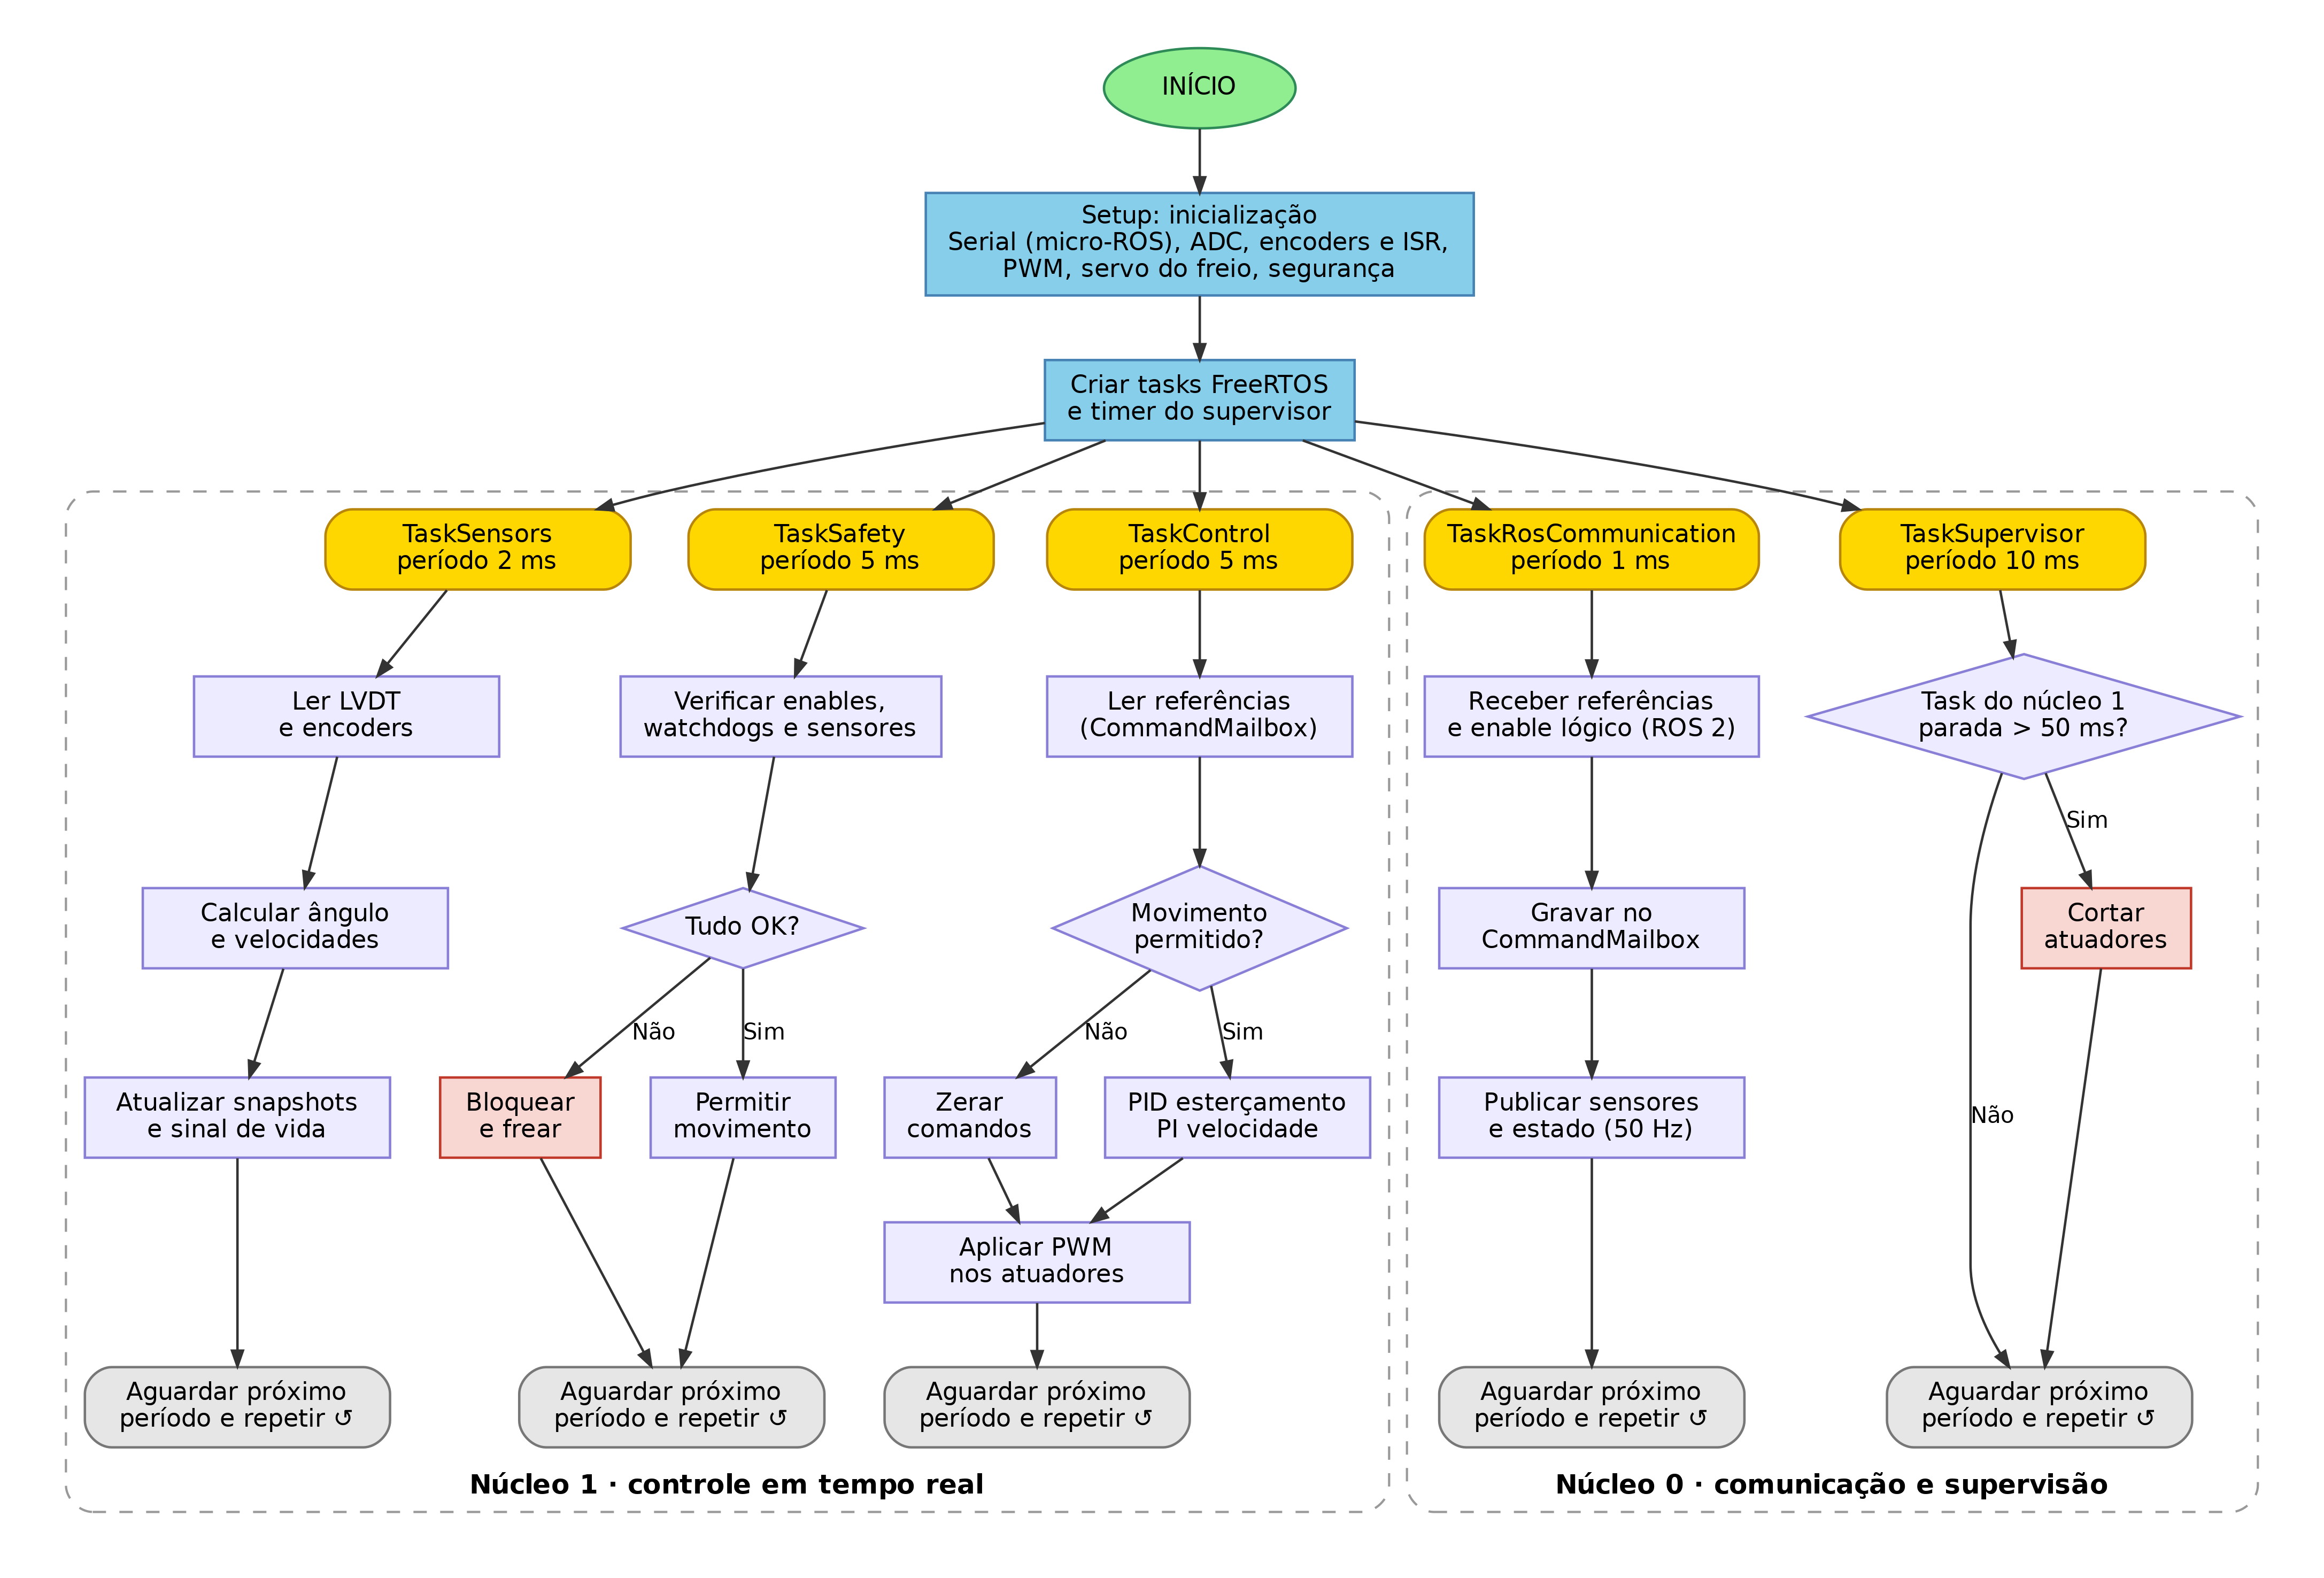
\includegraphics[width=\columnwidth]{Imagens/fluxograma_esp32.png}
    \caption{Diagrama das tarefas FreeRTOS no ESP32. Fonte: Elaborado pelo autor.}
    \label{fig:arquitetura_tasks_esp32}
\end{figure}

\subsection{Nível Intermediário -- Odroid N2}

O nível intermediário de processamento é constituído por um computador embarcado Odroid N2 com sistema operacional Linux, responsável pela integração do microcontrolador à infraestrutura ROS~2 e pela execução dos componentes de localização e estimação de estados do veículo.

Os ambientes de execução são organizados em dois containers Docker. O primeiro é dedicado ao agente micro-ROS, que estabelece a comunicação com o ESP32 e disponibiliza suas mensagens aos demais nós. O segundo reúne os nós executados no ROS~2 Humble: o driver do receptor GNSS, o cliente NTRIP, o estimador de estados e o nó de habilitação lógica.

O receptor GNSS u-blox ZED-F9R está conectado à Odroid por USB e fornece posições geográficas e medições da unidade inercial integrada. O cliente NTRIP, executado como um nó ROS~2, obtém as correções RTK de uma rede pública de estações de referência e as encaminha ao receptor pela mesma conexão USB, permitindo o posicionamento com precisão centimétrica. As posições GNSS são fundidas aos demais dados por meio de um filtro de Kalman estendido (EKF). A implementação do EKF é detalhada na Seção~\ref{sec:estimacao}.

A Odroid também executa o nó responsável por gerar o sinal de habilitação lógica enviado ao ESP32. Esse sinal permanece ativo enquanto o notebook recebe mensagens do controle de operação manual. A perda de comunicação com o operador, portanto, leva o ESP32 a bloquear o movimento e aplicar o freio.

A separação dos ambientes em containers isola as dependências do agente micro-ROS e dos demais componentes ROS~2, reduzindo conflitos de configuração efacilitando a manutenção e a atualização dos diferentes módulos.

\subsection{Nível de Alto Processamento -- Notebook}

O nível de alto processamento é executado em um notebook, responsável pelas funções de navegação, gerenciamento dos modos de operação e interação com o operador. Seus componentes de software são executados em ROS~2 Humble, organizado em container Docker, mantendo a compatibilidade com os demais dispositivos da arquitetura.

O sistema de navegação utiliza as estimativas do EKF para realizar o acompanhamento de uma trajetória previamente gravada com RTK. O controlador Stanley, é executado a cada nova estimativa de estado e sua implementação é detalhada na Seção~\ref{sec:seguimento_trajetoria}.

O notebook também executa o gerenciador de modos de operação, responsável por coordenar as transições entre a condução manual e a navegação autônoma, supervisionar as condições operacionais do veículo e encaminhar as referências de controle ao ESP32. O funcionamento desse gerenciador é detalhado na Seção~\ref{subsec:gerenciamento_navegacao}.

Para a condução manual, o operador utiliza um gamepad conectado ao notebook, cujos comandos são convertidos em referências de velocidade e de esterçamento e transmitidos pela mesma infraestrutura de comunicação utilizada no modo autônomo. Além disso, o notebook disponibiliza ferramentas para gravação e validação de trajetórias de referência e um painel de supervisão para o monitoramento do veículo.

A concentração dessas funções no notebook mantém os componentes de alto nível independentes das tarefas de aquisição e controle executadas nos demais dispositivos, facilitando a incorporação futura de algoritmos mais exigentes computacionalmente.


